%%=============================================================================
%% Methodologie
%%=============================================================================


\chapter{\IfLanguageName{dutch}{Methodologie}{Methodology}}%
\label{ch:methodologie}

%% TODO: In dit hoofstuk geef je een korte toelichting over hoe je te werk bent
%% gegaan. Verdeel je onderzoek in grote fasen, en licht in elke fase toe wat
%% de doelstelling was, welke deliverables daar uit gekomen zijn, en welke
%% onderzoeksmethoden je daarbij toegepast hebt. Verantwoord waarom je
%% op deze manier te werk gegaan bent.
%% 
%% Voorbeelden van zulke fasen zijn: literatuurstudie, opstellen van een
%% requirements-analyse, opstellen long-list (bij vergelijkende studie),
%% selectie van geschikte tools (bij vergelijkende studie, "short-list"),
%% opzetten testopstelling/PoC, uitvoeren testen en verzamelen
%% van resultaten, analyse van resultaten, ...
%%
%% !!!!! LET OP !!!!!
%%
%% Het is uitdrukkelijk NIET de bedoeling dat je het grootste deel van de corpus
%% van je bachelorproef in dit hoofstuk verwerkt! Dit hoofdstuk is eerder een
%% kort overzicht van je plan van aanpak.
%%
%% Maak voor elke fase (behalve het literatuuronderzoek) een NIEUW HOOFDSTUK aan
%% en geef het een gepaste titel.

Het doel van dit onderzoek is het identificeren van de meest geschikte pipeline voor de automatisering van het orderproces van een website naar 3D-geprinte producten. Dit proces zal iteratief verlopen, met fasen die zich richten op onderzoek, evaluatie, en prototyping. Elke fase heeft specifieke doelstellingen, deliverables en deadlines. Ook is het de bedoeling dat deze pipeline zal draaien op Mac en Windows.
\vspace{2em}

\textbf{Fase 1: Literatuurstudie}\\
\textbf{(Deadline: 07 maart 2025)}\\\\
In deze fase wordt er literatuuronderzoek gedaan naar bestaande oplossingen en pipelines die gebruikt kunnen worden voor de automatisering van het orderproces. Dit omvat een analyse van tools zoals Python, integraties met de Shopify API, en printbeheer API's zoals Bambu Studio. De deliverable voor deze fase is een lijst met mogelijke pipelines en tools die geschikt zouden kunnen zijn voor dit project, inclusief voor- en nadelen van elke optie.
\vspace{2em}

\textbf{Fase 2: Proof-of-Concept (PoC)}\\
\textbf{(Deadline: 4 april 2025)}\\\\
Op basis van de literatuurstudie worden meerdere pipelines geselecteerd en getest door een PoC op te zetten voor elke gekozen oplossing. Dit zal helpen om de haalbaarheid van de verschillende pipelines te testen. De PoC zal een order ontvangen via de Shopify API en doorsturen naar de Bambu Studio API. De technische haalbaarheid van elke pipeline wordt geëvalueerd om te bepalen welke het beste presteert.
\vspace{1em}

\textbf{Fase 3: Testen van de Pipelines en Prestatieanalyse}\\
\textbf{(Deadline: 18 April 2025)}\\\\
In deze fase worden de geselecteerde pipelines verder getest. Dit houdt in dat de pipelines onder verschillende belasting- en stressomstandigheden worden getest, zoals het verwerken van meerdere orders tegelijk. Daarnaast wordt er gekeken naar foutafhandelingsmechanismen en de stabiliteit van de integratie met de APIs. Enkele testscenario's omvatten: 
\begin{itemize}
    \item Wat gebeurt er als een bestand mislukt bij het verzenden?
    \item Wat gebeurt er als de printer zonder stroom valt?
    \item Wat gebeurt er bij een printfout?
    \item Hoe wordt het beëindigen van het printproces afgehandeld? 
\end{itemize}
\vspace{1em}

\textbf{Fase 4: Keuze van de Beste Pipeline en Optimalisatie}\\
\textbf{(Deadline: 25 april 2025)}\\\\
Na de uitvoerige tests wordt de beste pipeline geselecteerd op basis van prestaties, fouttolerantie en integratiegemak. In deze fase worden eventuele optimalisaties doorgevoerd en wordt de gekozen oplossing verder verfijnd voor de uiteindelijke implementatie.

\vspace{1em}
\textbf{Dit is de verwachte lijst van Tools:}\\
\begin{itemize}
    \item Python: voor het bouwen van de pipeline en het uitvoeren van API-aanroepen.
    \item Shopify API en Bambu Studio API: om orders te ontvangen en printopdrachten door te sturen.
    \item GitHub: voor versiebeheer van de code en documentatie.
    \item Postman: voor het testen van API-aanroepen tijdens de ontwikkeling.
    \item 3D-printer Bambu Lab X1C: voor het fysiek testen van het printproces.
    \item Verschillende pipelinetools: voor het opzetten en automatiseren van de integratie tussen de verschillende onderdelen van het systeem.
\end{itemize}

\vspace{1em}
\textbf{Dit is de verwachte lijst van functionele vereisten voor de applicatie:}
\\\\
Deze lijst is opgesteld op basis van de initiële projectdoelen en inzichten uit de literatuurstudie. Tijdens de Proof-of-Concept (Fase 2) en testfase (Fase 3) zullen deze vereisten geëvalueerd en indien nodig bijgesteld worden op basis van praktische haalbaarheid en testresultaten.
\\\\
\begin{itemize}
    \item \textbf{MUST}
    \begin{itemize}
        \item Order moet kunnen opgehaald worden  via de API.
        \item Juiste file moet kunnen opgehaald worden.
        \item Printopdracht moet kunnen gestart worden via de API.
    \end{itemize}
    \item \textbf{SHOULD}
    \begin{itemize}
        \item Communicatie naar eigenaar dat print gelsaagd is.
    \end{itemize}
    \item \textbf{COULD}
    \begin{itemize}
        \item Als meerdere orders binnenkomen deze samen plaatsen op het printbed indien mogelijk.
    \end{itemize}
\end{itemize}

\vspace{1em}
\textbf{Planning en deliverables}

\begin{itemize}
    \item Gemaakte flowchart
    
    \begin{figure}[H]  % Use [H] to prevent floating
        \centering
        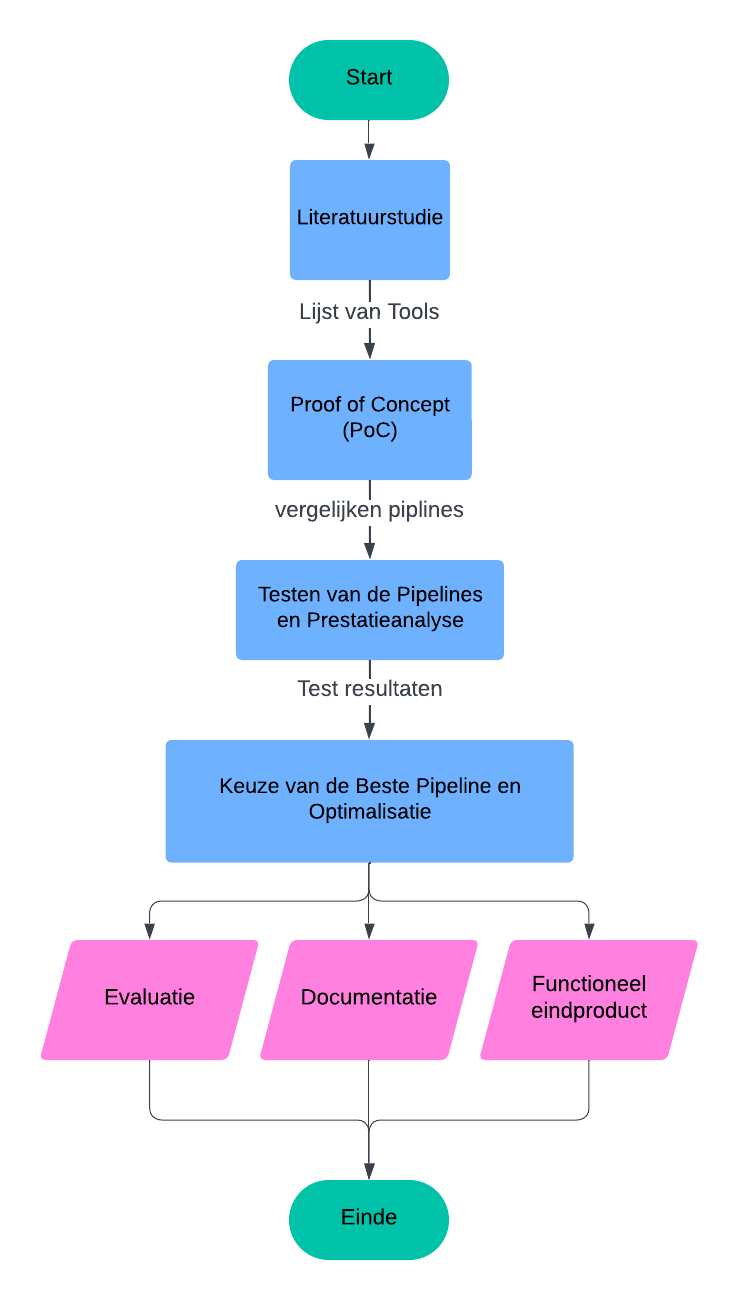
\includegraphics[width=0.5\textwidth]{Flowchart.png}  % Adjust width if necessary
        \caption{Flowchart van verschillende fasen en deliverables van de bachelorproef.}
        \label{fig:flowchart}  % Label for referencing
    \end{figure}
    
    \item Gemaakte Gantt chart.
    
    % Second figure: The Gantt Chart
    \begin{figure}[H]  % Use [H] to prevent floating
        \centering
        \resizebox{\textwidth}{!}{%
            \begin{ganttchart}[
                vgrid,
                hgrid,
                x unit=0.1cm,
                time slot format=isodate,
                compress calendar
                ]{2025-02-01}{2025-05-30}
                
                \gantttitlecalendar{year, month=name} \\
                
                % Fase 1: Literatuurstudie
                \ganttbar[
                progress=100,
                name=litstudie
                ]{Fase 1: Literatuurstudie}{2025-02-01}{2025-02-20} \\
                
                % Fase 2: Proof of Concept (PoC)
                \ganttbar[
                progress=0,
                name=poc
                ]{Fase 2: Proof-of-Concept}{2025-02-21}{2025-04-04} \\
                
                % Fase 3: Experimenten en Testen
                \ganttbar[
                progress=0,
                name=testen
                ]{Fase 3: Testen van de Pipelines en Prestatieanalyse}{2025-04-05}{2025-04-18} \\
                
                % Fase 4: Iteratieve Ontwikkeling en Optimalisatie
                \ganttbar[
                progress=0,
                name=optimalisatie
                ]{Fase 4: Keuze van de Beste Pipeline en Optimalisatie}{2025-04-19}{2025-04-25} \\
                
            \end{ganttchart}
        }
        \caption{Project Planning Gantt Chart}
        \label{fig:ganttchart}  % Label for referencing
    \end{figure}
\end{itemize}

\chapter{\IfLanguageName{dutch}{Proof-of-Concept}{Proof-of-Concept}}%
\label{ch:poc}

\section{Doel van deze fase}
Het doel van deze fase was het opzetten van een eerste werkende pipline tussen de webshop en de 3D-printer, ter validatie van de gekozen tools en technieken.

\section{Technische opstelling}
\begin{itemize}
    \item \textbf{Webshop:} Shopify met Webhook-integratie voor automatische orderdetectie.
    \item \textbf{3D-printer:} Creality Ender 3, aangestuurd via Raspberry Pi met MainsailOS + Moonraker API.
    \item \textbf{Communicatie:} Curl-commando’s naar Moonraker API voor slicen, uploaden en starten van printopdrachten.
    \item \textbf{Netwerktoegang:} Ngrok gebruikt om tijdelijk toegang te verlenen tot lokale services.
\end{itemize}

\section{Opmerkingen bij Bambu Lab Printer}
Initieel was het de bedoeling om de Bambu Lab X1C te gebruiken in combinatie met de Bambu Studio API. Door een software-update werd externe aansturing echter onmogelijk gemaakt zonder hun gesloten software. Daarom werd er overgeschakeld naar een open-source en lokaal beheersbare setup.

\section{CI/CD Tooling Evaluatie}
Om het automatiseringsproces te beheren en te testen, werden verschillende CI/CD tools onderzocht. Hieronder volgt een overzicht van de evaluatie:

\subsection{Geteste Tools}

\subsubsection{Jenkins (via Docker)}
\begin{itemize}
    \item \textbf{Voordelen:}
    \begin{itemize}
        \item Volledig lokaal hostbaar.
        \item Uitgebreide configuratiemogelijkheden via plugins.
        \item Volledige controle over netwerk en opslag.
        \item Geen problemen met authentificatie naar Moonraker.
    \end{itemize}
    \item \textbf{Nadelen:}
    \begin{itemize}
        \item Iets complexere setup (via Docker).
    \end{itemize}
\end{itemize}

\subsubsection{GitHub Actions}
\begin{itemize}
    \item \textbf{Voordelen:}
    \begin{itemize}
        \item Eenvoudige YAML-configuraties.
    \end{itemize}
    \item \textbf{Nadelen:}
    \begin{itemize}
        \item Enkel cloud-based, dus geen toegang tot lokaal netwerk of printers. (wel met ngrok)
        \item Vereist publieke poorten en authentificatie naar Moonraker.
        \item Veiligheidsrisico’s bij netwerktoegang.
    \end{itemize}
\end{itemize}

\subsubsection{GitLab CI/CD}
\begin{itemize}
    \item \textbf{Voordelen:}
    \begin{itemize}
        \item YAML-configuratie idem aan die van github actions met kleine aanpassingen.
        \item Self host gitlab runner dus kan lokaal gedraaid worden.
    \end{itemize}
    \item \textbf{Nadelen:}
    \begin{itemize}
        \item Vereist publieke poorten en authentificatie naar Moonraker. (online methode)
        \item Veiligheidsrisico’s bij netwerktoegang. (online methode)
        \item Maar 400 CI/CD minuten per maand.
    \end{itemize}
\end{itemize}

\subsection{Niet Geteste Tools}
Omwille van tijd door de bambulab update en kosten dat nodig zijn als je deze gebruikt op lange termijn, werden onderstaande tools niet verder onderzocht:
\begin{itemize}
    \item Bitbucket Pipelines
    \item Google Cloud Build
\end{itemize}

\section{Verwerking van een Order met Jenkins}
\begin{enumerate}
    \item Shopify stuurt via Webhook een order door.
    \item De juiste G-code wordt geselecteerd.
    \item Jenkins pipeline wordt getriggerd door de webhook.
    \item Commando’s worden via curl doorgestuurd naar Moonraker:
    \begin{itemize}
        \item \texttt{G28} commando om te 'homen'
        \item Upload naar MainsailOS
        \item Start van de printopdracht
    \end{itemize}
\end{enumerate}

\section{Stappenplan Uitgevoerde Oplossing}

Onderstaande stappen beschrijven het volledige opzet- en uitvoeringsproces van de PoC-oplossing waarbij een Shopify-webhook via Jenkins een 3D-printopdracht start op een Raspberry Pi met MainsailOS en Moonraker.

\subsection{Stap 1: Installaties en Voorbereidingen}
\begin{enumerate}
    \item Installeer \textbf{Docker} op je lokale machine.
    \item Installeer \textbf{Ngrok} om publieke toegang te voorzien naar je Jenkins-container.
    \item Installeer of maak een \textbf{Shopify-winkel} aan.
    \item Maak in Docker een aangepaste Jenkins-container aan:
    \begin{lstlisting}[language=bash, caption=Docker commando voor Jenkins met volume en poorten]
        docker run -d -p 8080:8080 -p 50000:50000 -v "D:\_3D_print_\Webshop:/var/jenkins_home" --name jenkins-met-backup jenkins-met-wijzigingen:custom
    \end{lstlisting}
    \item Open poort 8080 via Ngrok:
    \begin{lstlisting}[language=bash]
        ngrok http 8080
    \end{lstlisting}
    \item Start Jenkins en kopieer het initiële admin-wachtwoord uit de Docker terminal.
    \item Maak een admin account aan in de Jenkins UI.
    
    \item Installeer noodzakelijke Jenkins plugins:
    \begin{itemize}
        \item \texttt{Generic Webhook Trigger Plugin}
    \end{itemize}
\end{enumerate}

\vspace{0.5em}
\textit{Hier komt foto van: Docker Jenkins Container + Ngrok terminal output}

\subsection{Stap 2: Webhook Instellen in Shopify}
\begin{enumerate}
    \item Navigeer in Shopify naar \texttt{Instellingen > Meldingen > Webhooks}.
    \item Voeg een nieuwe webhook toe bij ``Bestelling aangemaakt''.
    \item Stel de webhook-URL in als volgt:
    \begin{lstlisting}[language=text]
        https://<jouw-ngrok-url>/generic-webhook-trigger/invoke?token=shopify-jenkins-trigger
    \end{lstlisting}
    \item Kies als indeling: \texttt{JSON}.
\end{enumerate}

\vspace{0.5em}
\textit{Hier komt screenshot van: Shopify webhook-configuratie}

\subsection{Stap 3: Aanmaken Jenkins Pipeline}
\begin{enumerate}
    \item Maak een nieuw Pipeline-project aan in Jenkins.
    \item Koppel het project aan een GitHub-repository.
    \item Voeg een \texttt{Jenkinsfile} toe in de repo met volgende inhoud:

\subsection*{Stap 1: Shopify trigger naar Jenkins}

Een \texttt{Generic Webhook Trigger} plugin wordt gebruikt in Jenkins om inkomende bestellingen te detecteren. Hieronder zie je het deel van de configuratie dat de trigger mogelijk maakt:

\begin{lstlisting}[language=groovy, caption=Webhook-trigger configuratie in Jenkinsfile]
    triggers {
        GenericTrigger(
        genericVariables: [
        [key: 'order_id', value: '$.id'],
        [key: 'product_names', value: '$.line_items[*].name', expressionType: 'JSONPath']
        ],
        token: 'shopify-jenkins-trigger'
        )
    }
\end{lstlisting}

\subsection*{Stap 2: Controle van het bestandsvolume}

Vooraleer een printopdracht wordt verstuurd, wordt nagegaan of het juiste G-code bestand bestaat in de Jenkins container (via een Docker volume gekoppeld aan de host).

\begin{lstlisting}[language=groovy, caption=Controle van Jenkins volume]
    stage('Check File System') {
        steps {
            sh 'ls -la /var/jenkins_home'
        }
    }
\end{lstlisting}

\subsection*{Stap 3: Informatie over de bestelling loggen}

Bij het ontvangen van de bestelling loggen we de producten zodat we later kunnen debuggen of analyseren wat er is binnengekomen.

\begin{lstlisting}[language=groovy, caption=Debugging van de ontvangen productnamen]
    stage('Debug Bestelling') {
        steps {
            echo "Ontvangen productnamen: ${env.product_names}"
        }
    }
\end{lstlisting}

\subsection*{Stap 4: Voorbereiding van het G-code bestand}

We selecteren één product en controleren of het bijhorende .gcode bestand klaarstaat om geprint te worden:

\begin{lstlisting}[language=groovy, caption=Controleren van G-code beschikbaarheid]
    stage('Prepare G-code') {
        steps {
            script {
                def order_name = env.product_names.replaceAll("[\\[\\]\" ]", "").split(",")[0]
                def gcodeFilePath = "/var/jenkins_home/${order_name}.gcode"
                if (!fileExists(gcodeFilePath)) {
                    error "G-code niet gevonden: ${gcodeFilePath}"
                }
            }
        }
    }
\end{lstlisting}

\subsection*{Stap 5: Verzenden van de printopdracht}

Zodra alles correct is voorbereid, worden via CURL-commando’s drie instructies naar de printer gestuurd:

\begin{enumerate}
    \item \textbf{G28} om de printer te 'homing'.
    \item Upload van het G-code bestand.
    \item Starten van het printproces.
\end{enumerate}

\begin{lstlisting}[language=groovy, caption=Starten van het printproces via curl]
    stage('Start Print') {
        steps {
            script {
                sh '''curl -X POST .../printer/gcode/script -d '{"script": "G28"}' '''
                sh '''curl -X POST .../server/files/upload -F "file=@..." '''
                sh '''curl -X POST .../printer/print/start -d '{"filename": "..."}' '''
            }
        }
    }
\end{lstlisting}


\vspace{0.5em}
\textit{Hier komt screenshot van: Jenkins-pipeline configuratie met webhook trigger}

\subsection{Stap 4: Bestandenstructuur en G-code}
\begin{itemize}
    \item De G-code bestanden worden lokaal bewaard in de Jenkins volume map: \texttt{/var/jenkins\_home/}.
    \item De naam van het bestand moet overeenkomen met het ontvangen product via Shopify.
\end{itemize}

\vspace{0.5em}
\textit{Hier komt screenshot van: bestand in map \texttt{jenkins\_home} zichtbaar via Jenkins console}

\subsection{Stap 5: Printer Instellingen}
\begin{itemize}
    \item Raspberry Pi draait MainsailOS met Moonraker.
    \item Printer is lokaal bereikbaar via IP: \texttt{192.168.1.100:7125}.
    \item Curl-commando’s sturen G-code naar de printer.
    \item Volgorde: Homen met \texttt{G28} → uploaden → print starten.
\end{itemize}

\vspace{0.5em}
\textit{Hier komt foto van: Raspberry Pi + printer setup}

\subsection{Afweging .py-scripts vs Curl}
Tijdens de PoC is gebleken dat het gebruik van rechtstreekse \texttt{curl}-commando’s eenvoudiger en sneller resultaat gaf dan Python-scripts met externe libraries zoals \texttt{moonrakerpy}. Hierdoor werd gekozen om tijdens de PoC te werken met directe API-aanroepen.

\subsection{Afsluitende Opmerkingen}
\begin{itemize}
    \item Niet alle packages in \texttt{requirements.txt} werden effectief gebruikt.
    \item Voor productie is het aangeraden om Jenkins lokaal op een Raspberry Pi te hosten i.p.v. via Ngrok.
    \item Curl biedt betrouwbaardere controle tijdens testen dan afhankelijkheden van externe libraries.
\end{itemize}

\section{Besluit}
Op basis van de uitgevoerde tests is \textbf{Jenkins} geselecteerd als meest geschikte tool voor verdere uitwerking. Belangrijke redenen zijn:
\begin{itemize}
    \item Volledig lokaal beheer.
    \item Flexibiliteit en uitbreidbaarheid.
    \item Geen externe afhankelijkheden of veiligheidsrisico’s.
\end{itemize}

Er is beslist om de Jenkins-oplossing verder te optimaliseren in de volgende fase van het project.





